
\subsection{Proof of Lemma~\ref{lemma_actives_sets}}

Since the objective function $\Psi_{\kappa}$ is convex with respect to $(u,v)$, the set of optima of problem~\eqref{screen-sinkhorn} is non empty.
Introducing two dual variables $\lambda \in \R^n_{+}$ and $\beta \in \R^m_{+}$ for each constraint, the Lagrangian of problem~\eqref{screen-sinkhorn} reads as 
\begin{equation*}
  \mathscr{L}(u,v, \lambda, \beta) = \frac \varepsilon\kappa\inr{\lambda, \mathbf{1}_n} + \varepsilon\kappa\inr{\beta, \mathbf{1}_m} + \mathbf{1}_n^\top B(u,v) \mathbf{1}_m - \inr{\kappa u, \mu} - \inr{\frac v\kappa, \nu} -\inr{\lambda,e^{u}} - \inr{\beta,e^{v}}
\end{equation*}
First order conditions then yield that the Lagrangian multiplicators solutions $\lambda^{*}$ and $\beta^{*}$ satisfy 
\begin{align*}
  &\nabla_u\mathscr{L}(u^{*},v^{*}, \lambda^{*}, \beta^{*})=  e^{u^{*}} \odot(Ke^{v^{*}} - \lambda^{*}) - \kappa\mu = \mathbf 0_n,\\
  & \text{ and } \nabla_v\mathscr{L}(u^{*},v^{*}, \lambda^{*}, \beta^{*})=  e^{v^{*}} \odot(K^\top e^{u^{*}} - \beta) - \frac \nu\kappa = \mathbf 0_m
\end{align*}
which leads to 
\begin{align*}
  &\lambda^{*} = K e^{v^{*}} - \kappa\mu \oslash e^{u^{*}} \text{ and }
  \beta^{*} = K^\top e^{u^{*}} - \nu \oslash \kappa e^{v^{*}}
\end{align*}

For all $i=1, \ldots, n$ we have that $e^{u^{*}_i} \geq \varepsilon\kappa^{-1}$. Further, the condition on the dual variable $\lambda^{*}_i > 0$  ensures that $e^{u^{*}_i} = \varepsilon\kappa^{-1}$ and hence $i \in I^\complement_{\varepsilon,\kappa}$. We have that $\lambda^{*}_i > 0$ is equivalent to $e^{u^{*}_i}r_i(K) e^{v^{*}_j} >  \kappa{\mu_i}$ which  is satisfied when $\varepsilon^2r_i(K) >  \kappa{\mu_i}.$  
In a symmetric way we can prove the same statement for $e^{v^{*}_j}$.

\subsection{Proof of Proposition~\ref{prop:bounds_of_usc_and_vsc}}

We prove only the first statement~\eqref{bound_on_u} and similarly we can prove the second one~\eqref{bound_on_v}.
For all $i\in I_{\varepsilon,\kappa}$, we have $e^{u^{\text{sc}}_i} > \frac \varepsilon\kappa$ or $e^{u^{\text{sc}}_i} = \frac \varepsilon\kappa$. In one hand, if $e^{u^{\text{sc}}_i} > \frac \varepsilon\kappa$ then according to the optimality conditions $\lambda^{\text{sc}}_i = 0,$ which implies $e^{u^{\text{sc}}_i} \sum_{j=1}^m K_{ij} e^{v^{\text{sc}}_j} = \kappa\mu_i$.
In another hand, we have 
\begin{align*}
e^{u^{\text{sc}}_i} \min_{i,j}K_{ij} \sum_{j=1}^m e^{v^{\text{sc}}_j} \leq e^{u^{\text{sc}}_i} \sum_{j=1}^m K_{ij} e^{v^{\text{sc}}_j} = \kappa\mu_i.
\end{align*}
We further observe that $\sum_{j=1}^m e^{v^{\text{sc}}_j} = \sum_{j \in J_{\varepsilon,\kappa}} e^{v^{\text{sc}}_j} + \sum_{j \in J^\complement_{\varepsilon,\kappa}} e^{v^{\text{sc}}_j} \geq \varepsilon\kappa |J_{\varepsilon,\kappa}| + \varepsilon\kappa |J^\complement_{\varepsilon,\kappa}|=\varepsilon\kappa m.$ Then
\begin{equation*}
\max_{i\in I_{\varepsilon,\kappa}} e^{u^{\text{sc}}_i} \leq \frac \varepsilon\kappa \vee \frac{\max_{i\in I_{\varepsilon,\kappa}}\mu_i}{m\varepsilon K_{\min}} \leq \frac \varepsilon\kappa \vee \frac{\max_{i\in I_{\varepsilon,\kappa}}\mu_i}{m\varepsilon K_{\min}}.
\end{equation*}
Analogously, one can obtain for all $j\in J_{\varepsilon,\kappa}$
\begin{equation}
\label{upper_bound_v_potential}
\max_{j\in J_{\varepsilon,\kappa}}e^{v^{\text{sc}}_j} \leq \varepsilon\kappa \vee \frac{\max_{j \in J_{\varepsilon,\kappa}} \nu_j}{n\varepsilon K_{\min}} \leq \varepsilon\kappa \vee \frac{\max_{j \in J_{\varepsilon,\kappa}} \nu_j}{n\varepsilon K_{\min}} .
\end{equation}

Now, since $K_{ij} \leq 1$, we have 
\begin{align*}
e^{u^{\text{sc}}_i} \sum_{j=1}^m e^{v^{\text{sc}}_j} \geq e^{u^{\text{sc}}_i} \sum_{j=1}^m K_{ij}e^{v^{\text{sc}}_j} = \kappa\mu_i.
\end{align*}
Using~\eqref{upper_bound_v_potential}, we get 
\begin{align*}
\sum_{j=1}^m e^{v^{\text{sc}}_j} &= \sum_{j \in J_{\varepsilon,\kappa}} e^{v^{\text{sc}}_j} + \sum_{j \in J^\complement_{\varepsilon,\kappa}} e^{v^{\text{sc}}_j}
\leq \varepsilon\kappa |J^\complement_{\varepsilon,\kappa}| + \varepsilon\kappa \vee \frac{\max_{j\in J_{\varepsilon,\kappa}} \nu_j}{n\varepsilon K_{\min}} |J_{\varepsilon,\kappa}|.
\end{align*}
Therefore,
\begin{align*}
\min_{i \in I_{\varepsilon,\kappa}} e^{u^{\text{sc}}_i}  \geq \frac \varepsilon\kappa \vee \frac{\kappa\min_{I_{\varepsilon,\kappa}}\mu_i}{\varepsilon\kappa (m-m_b) + \varepsilon\kappa \vee \frac{\max_{j\in J_{\varepsilon,\kappa}} \nu_j}{n\varepsilon K_{\min}} m_b}.
\end{align*}

\subsection{Proof of Lemma~\ref{lemma_bounds_on_marginals}}


The optimality condition for $({u}^{\text{sc}}, {v}^{\text{sc}})$ entails 
\begin{align}
\label{i-th-marginal-mu} 
{\mu}^{\text{sc}}_i  &= 
\begin{cases}
e^{u^{\text{sc}}_i} \sum_{j=1}^m K_{ij} e^{v^{\text{sc}}_j}, \text{ if  }i \in I_{\varepsilon,\kappa},\\
\frac \varepsilon\kappa\sum_{j=1}^m K_{ij} e^{v^{\text{sc}}_j}, \text{ if  }i \in I^\complement_{\varepsilon,\kappa}
\end{cases}
=\begin{cases}
\kappa \mu_i, \text{ if  }i \in I_{\varepsilon,\kappa},\\
\frac \varepsilon\kappa\sum_{j=1}^m K_{ij} e^{v^{\text{sc}}_j}, \text{ if  }i \in I^\complement_{\varepsilon,\kappa},
\end{cases}
\end{align}
and 
\begin{align}
\label{i-th-marginal-nu} 
{\nu}^{\text{sc}}_j  &= 
\begin{cases}
e^{v^{\text{sc}}_j} \sum_{i=1}^n K_{ij} e^{u^{\text{sc}}_i}, \text{ if  }j \in J_{\varepsilon,\kappa},\\
\varepsilon\kappa\sum_{i=1}^n K_{ij} e^{u^{\text{sc}}_i}, \text{ if  }j \in J^\complement_{\varepsilon,\kappa}
\end{cases}
=\begin{cases}
\frac{\nu_j}{\kappa}, \text{ if  }j \in J_{\varepsilon,\kappa},\\
\varepsilon\kappa\sum_{i=1}^n K_{ij} e^{u^{\text{sc}}_i}, \text{ if  }j \in J^\complement_{\varepsilon,\kappa}.
\end{cases}
\end{align}

Using inequality~\eqref{bound_on_v}, we obtain 
\begin{align*}
\norm{\mu^{\text{sc}}}_1 &= \sum_{i \in I_{\varepsilon,\kappa}} \mu^{\text{sc}}_i +  \sum_{i \in I^\complement_{\varepsilon,\kappa}}\mu^{\text{sc}}_i\\
& \overset{\eqref{i-th-marginal-mu}}{=} \kappa \norm{\mu_{I_{\varepsilon,\kappa}}^{\text{sc}}}_1 + \frac \varepsilon\kappa \sum_{i \in I^\complement}\Big( \sum_{j \in J_{\varepsilon,\kappa}} K_{ij} e^{v^{\text{sc}}_j} + \varepsilon\kappa \sum_{j\in J^\complement_{\varepsilon,\kappa}}K_{ij}\Big)\\
& \overset{\eqref{bound_on_v}}{\leq} \kappa \norm{\mu_{I_{\varepsilon,\kappa}}^{\text{sc}}}_1 + (n-n_b) \Big(\frac{m_b\max_{j \in J_{\varepsilon,\kappa}} \nu_j}{n\kappa K_{\min}} + (m-m_b)\varepsilon^2 \Big).
\end{align*}
Again by left-hand-side of inequaltiy~\eqref{bound_on_v}, we arrive at 
\begin{align*}
\norm{\mu^{\text{sc}}}_1 %&= \sum_{i \in I_{\varepsilon,\kappa}} \mu^{\text{sc}}_i +  \sum_{i \in I^\complement_{\varepsilon,\kappa}}\mu^{\text{sc}}_i\\
%& \overset{\eqref{i-th-marginal-mu}}{=} \kappa \norm{\mu_{I_{\varepsilon,\kappa}}^{\text{sc}}}_1 + \frac \varepsilon\kappa \sum_{i \in I^\complement}\Big( \sum_{j \in J_{\varepsilon,\kappa}} K_{ij} e^{v^{\text{sc}}_j} + \varepsilon\kappa \sum_{j\in J^\complement_{\varepsilon,\kappa}}K_{ij}\Big)\\
& \overset{}{\geq} \kappa \norm{\mu_{I_{\varepsilon,\kappa}}^{\text{sc}}}_1 + (n -n_b) \Big(\frac{mm_b\varepsilon^2 K_{\min}^2 \min_{j\in J_{\varepsilon, \kappa}} \nu_j}{ (n-n_b)m\kappa \varepsilon^2 K_{\min} + n_b\kappa^2 \max_{i\in I_{\varepsilon,\kappa}}\mu_i }+ (m-m_b)\varepsilon^2K_{\min}\Big),
\end{align*}
which gives the claimed result.
Similarly, we can prove the same statement for $\norm{\nu^{\text{sc}}}_1$.

\subsection{Proof of Proposition~\ref{proposition_error_in_marginals}}

We define the distance function $\varrho: \R_+ \times \R_+ \mapsto [0, \infty]$ by $\varrho(a,b) = b - a + a \log(\frac ab).$
While $\varrho$ is not a metric, it is easy to see that $\varrho$ is not nonnegative and satisfies $\varrho(a,b) =0$ iff $a=b$.
The violations are computed through the following function: 
\begin{equation*}
	d_{\varrho}(\gamma,\beta) = \sum_{i=1}^n \varrho(\gamma_i,\beta_i), \text{ for } \gamma, \beta \in \R^n_+.
\end{equation*}
Note that if $\gamma,\beta$ are two vectors of positive entries, $d_{\varrho}(\gamma,\beta)$ will return some measurement on how far they are from each other. The next Lemma is from~\cite{khalilabid2018} (see Lemma 7 herein).
\begin{lemma}
\label{lem:pinsker}
For any $\gamma, \beta \in \R^n_+$, the following generalized Pinsker inequality holds 
\begin{align*}
\norm{\gamma - \beta}_1 \leq \sqrt{7 (\norm{\gamma}_1\wedge \norm{\beta}_1)d_{\varrho}(\gamma,\beta)}
\end{align*}
\end{lemma}
By~\eqref{i-th-marginal-mu}, we have
\begin{align*}
d_\varrho({\mu} ,{\mu}^{\text{sc}}) &= \sum_{i=1}^n  {\mu}^{\text{sc}}_i - {\mu}_i + {\mu}_i  \log\Big(\frac{{\mu}_i}{{\mu}^{\text{sc}}_i }\Big)\\
&= \sum_{i\in I_{\varepsilon,\kappa}} (\kappa-1)\mu_i - \mu_i\log(\kappa) + \sum_{i\in I^\complement_{\varepsilon,\kappa}}\frac \varepsilon\kappa\sum_{j=1}^m K_{ij} e^{v^{\text{sc}}_j} - \mu_i + \mu_i \log\Big(\frac{\mu_i}{\frac \varepsilon\kappa\sum_{j=1}^m K_{ij} e^{v^{\text{sc}}_j}}\Big)\\
&= \sum_{i\in I_{\varepsilon,\kappa}} (\kappa-\log(\kappa)-1)\mu_i  + \sum_{i\in I^\complement_{\varepsilon,\kappa}}\frac \varepsilon\kappa\sum_{j=1}^m K_{ij} e^{v^{\text{sc}}_j} - \mu_i + \mu_i \log\Big(\frac{\mu_i}{\frac \varepsilon\kappa\sum_{j=1}^m K_{ij} e^{v^{\text{sc}}_j}}\Big).
% &\leq  \sum_{i\in I^\complement_{\varepsilon,\kappa}}\frac \varepsilon\kappa\sum_{j=1}^m K_{ij} e^{v^{\text{sc}}_j} - \mu_i + \mu_i \log\Big(\frac{\mu_i}{\frac \varepsilon\kappa\sum_{j=1}^m K_{ij} e^{v^{\text{sc}}_j}}\Big)
\end{align*}
Now by~\eqref{bound_on_v}, we have in one hand 
\begin{align*}
\sum_{i\in I^\complement_{\varepsilon,\kappa}}\frac \varepsilon\kappa\sum_{j=1}^m K_{ij} e^{v^{\text{sc}}_j}&= \sum_{i\in I^\complement_{\varepsilon,\kappa}}\frac \varepsilon\kappa \Big(\sum_{j\in J_{\varepsilon,\kappa}}K_{ij} e^{v^{\text{sc}}_j} + \varepsilon \kappa\sum_{j\in J^\complement_{\varepsilon,\kappa}}K_{ij}\Big)\\
&\leq \sum_{i\in I^\complement_{\varepsilon,\kappa}}\frac \varepsilon\kappa \Big(m_b \max_{i,j}K_{ij}\frac{\max_{j \in J_{\varepsilon,\kappa}} \nu_j}{n\varepsilon K_{\min}} + (m - m_b)\varepsilon\kappa\max_{i,j}K_{ij}\Big) \\
&\leq (n-n_b)\Big(\frac{m_b\max_{j} \nu_j}{n\kappa K_{\min}} + (m- m_b) \varepsilon^2\Big).
\end{align*}
On the other hand, we get
\begin{align*}
\frac \varepsilon\kappa\sum_{j=1}^m K_{ij} e^{v^{\text{sc}}_j}&=\frac \varepsilon\kappa \Big(\sum_{j\in J_{\varepsilon,\kappa}}K_{ij} e^{v^{\text{sc}}_j} + \varepsilon \kappa\sum_{j\in J^\complement_{\varepsilon,\kappa}}K_{ij}\Big)\\
&\geq m_bK_{\min} \frac{m\varepsilon^2K_{\min}\min_{j \in J_{\varepsilon,\kappa}}\nu_j}{\kappa((n-n_b)m\varepsilon^2K_{\min} + m\varepsilon^2K_{\min} + n_b\kappa\max_{i\in I_{\varepsilon,\kappa}}\mu_i)}\\
&\qquad +\varepsilon^2 (m- m_b) K_{\min}\\
&\geq \frac{mm_b\varepsilon^2(K_{\min})^2\min_{j \in J_{\varepsilon,\kappa}}\nu_j}{\kappa((n-n_b)m\varepsilon^2K_{\min}+ m\varepsilon^2K_{\min} + n_b\kappa\max_{i\in I_{\varepsilon,\kappa}}\mu_i)}\\
&\qquad +\varepsilon^2 (m- m_b) K_{\min}\\
&\geq \frac{mm_b\varepsilon^2K_{\min}^2\min_{j \in J_{\varepsilon,\kappa}}\nu_j}{\kappa((n-n_b)m\varepsilon^2K_{\min}+ m\varepsilon^2K_{\min} + n_b\kappa\max_{i\in I_{\varepsilon,\kappa}}\mu_i)}.
\end{align*}
Then 
\begin{align*}
\frac{1}{\frac \varepsilon\kappa\sum_{j=1}^m K_{ij} e^{v^{\text{sc}}_j}} &\leq \frac{\kappa((n-n_b)m\varepsilon^2K_{\min}+ m\varepsilon^2K_{\min} + n_b\kappa\max_{i\in I_{\varepsilon,\kappa}}\mu_i)}{mm_b\varepsilon^2 K_{\min}^2\min_{j \in J_{\varepsilon,\kappa}}\nu_j}\\
&\leq \frac{\kappa(n-n_b+ 1)}{m_bK_{\min}\min_{j \in J_{\varepsilon,\kappa}}\nu_j} + \frac{n_b\kappa^2\max_{i\in I_{\varepsilon,\kappa}}\mu_i}{mm_b\varepsilon^2K_{\min}^2\min_{j \in J_{\varepsilon,\kappa}}\nu_j}.
\end{align*}
It entails 
\begin{align*}
&\sum_{i\in I^\complement_{\varepsilon,\kappa}}\frac \varepsilon\kappa\sum_{j=1}^m K_{ij} e^{v^{\text{sc}}_j} - \mu_i + \mu_i \log\Big(\frac{\mu_i}{\frac \varepsilon\kappa\sum_{j=1}^m K_{ij} e^{v^{\text{sc}}_j}}\Big)\\
&\leq (n-n_b)\bigg(\frac{m_b}{n\kappa\min_{i,j} K_{ij}} + (m- m_b) \varepsilon^2 - \min_{i}\mu_i\\
&\qquad + \max_{i}\mu_i\log\Big(\frac{\kappa(n-n_b+ 1)\max_{i}\mu_i}{m_bK_{\min}\min_{j \in J_{\varepsilon,\kappa}}\nu_j} + \frac{n_b\kappa^2(\max_{i}\mu_i)^2}{mm_b\varepsilon^2 K_{\min}^2\min_{j \in J_{\varepsilon,\kappa}}\nu_j}\Big)
\bigg).
\end{align*}
Therefore
\begin{align*}
d_\varrho({\mu},{\mu}^{\text{sc}}) &\leq n_b(\kappa-\log(\kappa)-1)\max_{i} \mu_i + (n-n_b)\bigg(\frac{m_b\max_{j}\nu_j}{n\kappa\min_{i,j} K_{ij}} + (m- m_b) \varepsilon^2 - \min_{i}\mu_i\\
&\qquad + \max_{i} \mu_i\log\Big(\frac{\kappa(n-n_b+ 1)\max_{i} \mu_i}{m_bK_{\min}\min_{j \in J_{\varepsilon,\kappa}}\nu_j} + \frac{n_b\kappa^2(\max_{i} \mu_i)^2}{mm_b\varepsilon^2 K_{\min}^2\min_{j \in J_{\varepsilon,\kappa}}\nu_j}\Big).
\end{align*}
Finally, by Lemma~\ref{lem:pinsker} we obtain
\begin{align*}
\norm{{\mu} -{\mu}^{\text{sc}}}^2_1 \leq & n_b(\kappa-\log(\kappa)-1)\max_{i} \mu_i + 7(n-n_b)\bigg(\frac{m_b\max_{j}\nu_j}{n\kappa\min_{i,j} K_{ij}} + (m- m_b) \varepsilon^2 - \min_{i}\mu_i\\
&+ \max_{i} \mu_i\log\Big(\frac{\kappa(n-n_b+ 1)\max_{i} \mu_i}{m_bK_{\min}\min_{j \in J_{\varepsilon,\kappa}}\nu_j} + \frac{n_b\kappa^2(\max_{i} \mu_i)^2}{mm_b\varepsilon^2K_{\min}^2\min_{j \in J_{\varepsilon,\kappa}}\nu_j}\Big).%\bigg\}^{1/2}
\end{align*}
Proof of the upper bound for $\norm{\nu - {\nu}^{\text{sc}}}^2_1$ follows the same lines as above.



\subsection{Additional experimental results}


\begin{figure*}[t]
	\centering
	
	\includegraphics[width=6.cm]{../../figure/da_gain_toy_regcl1.pdf}
	\includegraphics[width=6.cm]{../../figure/da_gain_toy_regcl10.pdf}
	\includegraphics[width=6.cm]{../../figure/da_accur_toy_regcl1.pdf}
	\includegraphics[width=6.cm]{../../figure/da_accur_toy_regcl10.pdf}
	\caption{OT Domain Adaptation on a toy problem : running time gain for a toy dataset and for mnist as a function of the number of examples and the data decimation factor in \emph{Screenkhorn}}.
	\label{fig:otda}
\end{figure*}


\begin{figure*}[t]
	\centering
	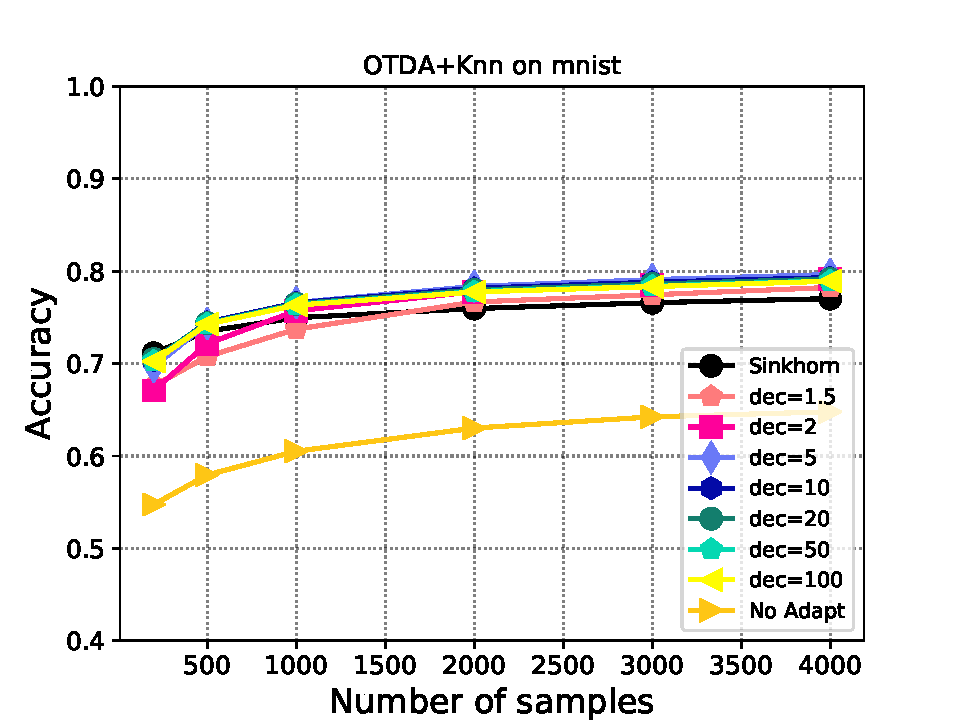
\includegraphics[width=6.5cm]{../../figure/da_accur_mnist_regcl1.pdf}
	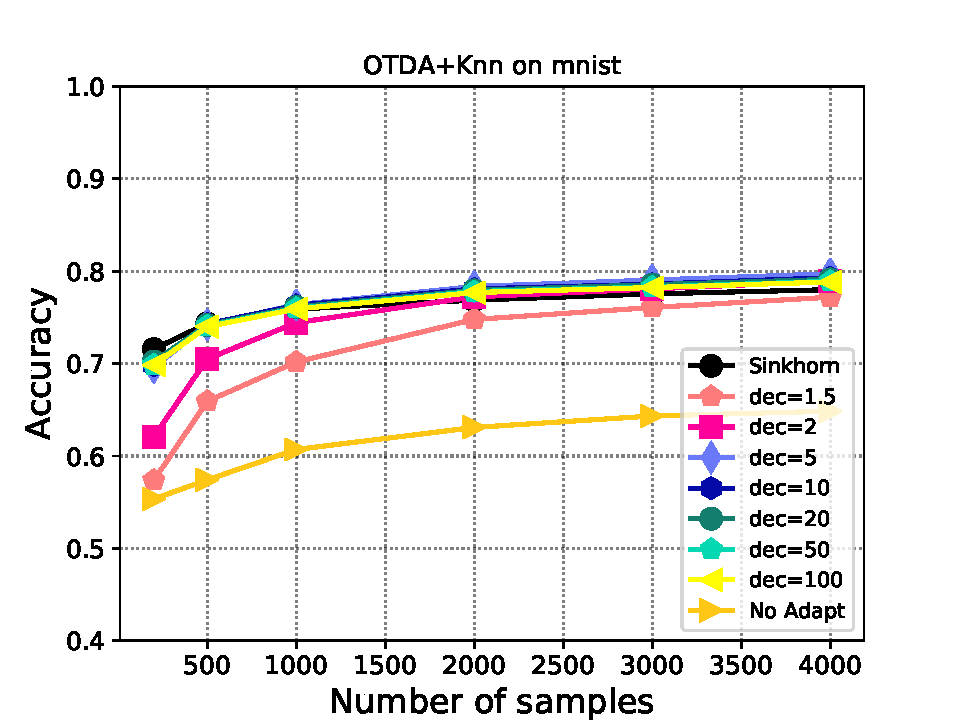
\includegraphics[width=6.5cm]{../../figure/da_accur_mnist_regcl10.pdf}
	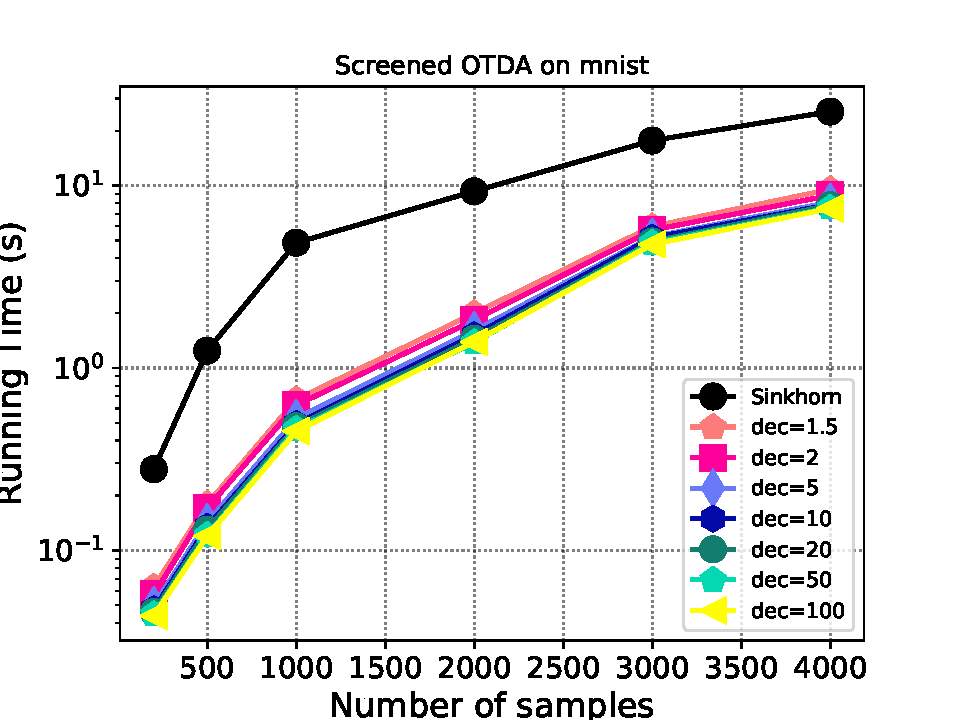
\includegraphics[width=6.5cm]{../../figure/da_time_mnist_regcl1.pdf}
	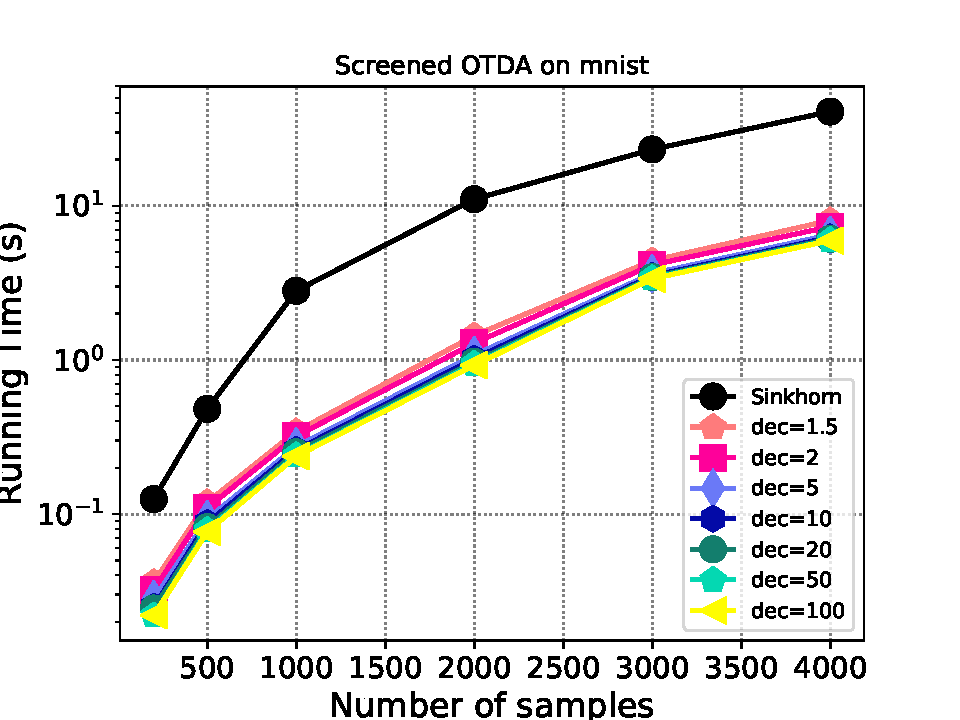
\includegraphics[width=6.5cm]{../../figure/da_time_mnist_regcl10.pdf}
	\caption{OT Domain adaptation MNIST to USPS : (top) Accuracy and (bottom) running time of Sinkhorn and \emph{Screenkhorn} for hyperparameter of the $\ell_{p,1}$ regularizer (left) $\lambda = 1$ and (right) $\lambda=10$. Note that this
	value impact of the ground cost of each Sinkhorn problem involved in the iterative algorithm. The accuracy panels
	also report the performance of a $1$-NN when no-adaptation is performed.  
	We remark that the strenght of the class-based has influence on the performance of \emph{Screenkhorn} given a decimation factor. For small value on the left, Screenkhorn slightly performs better than Sinkhorn, while for large value, some
	decimation factors leads to loss of performances.
	Regarding, running time, we can note that Sinkhorn is far less efficient than
	\emph{Screenkhorn}  with an order of magnitude for intermediate number of samples.
	\label{fig:otda:mnist:extra}}
\end{figure*}